\begin{scanpage}{0228}{210}
\noindent\begin{minipage}[t]{.47\linewidth}\vspace{0pt}
\vspace{35pt}\centering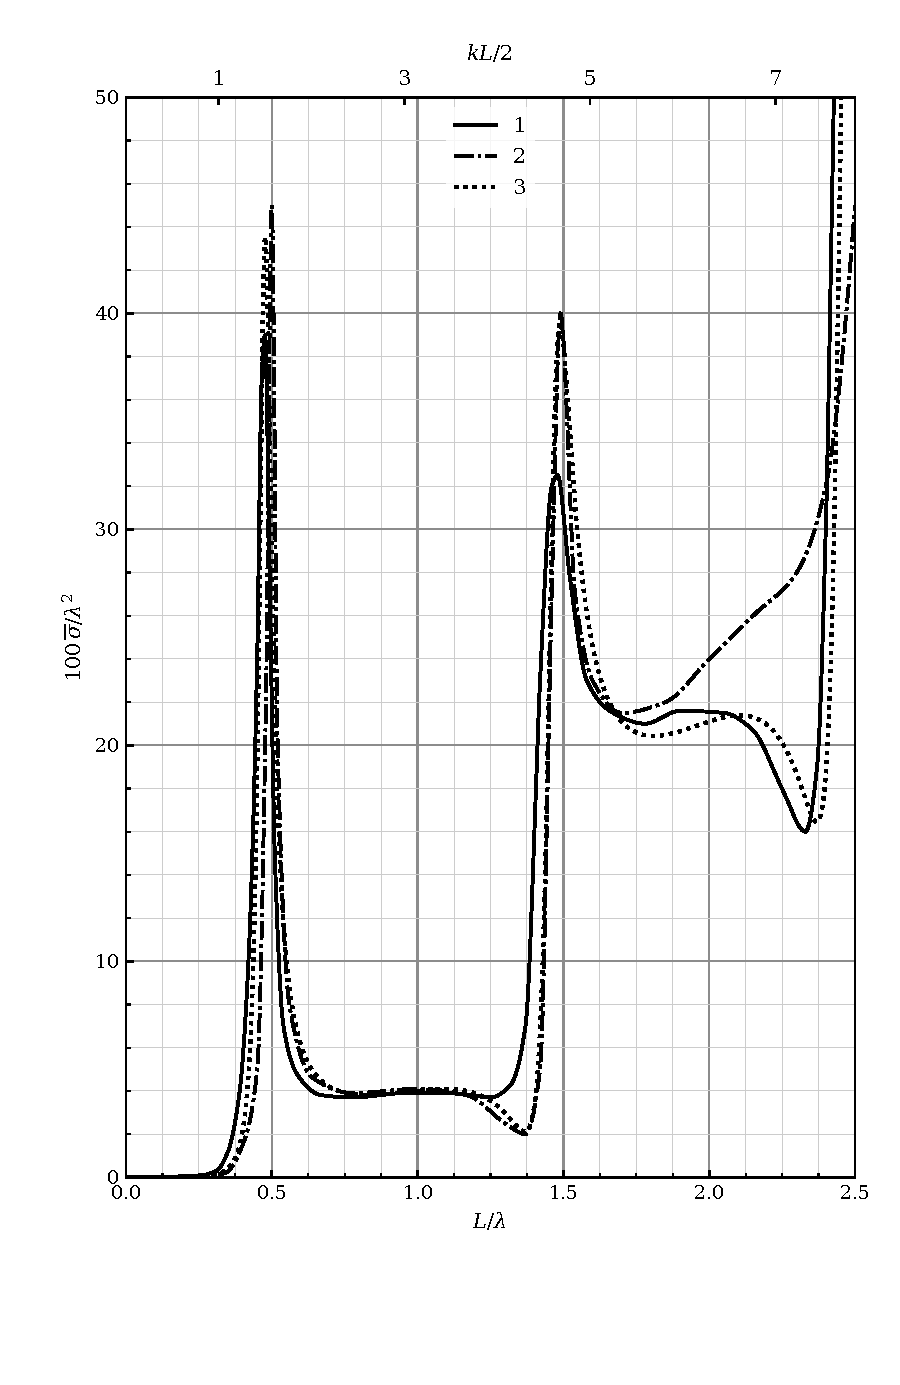
\includegraphics[width=.95\linewidth]{images/recreated/r-0228-fig77.pdf}\par\medskip
\raggedright Figure 77. The effective scattering area of a vibrator as a function of its length with normal incidence of a plane wave. Curve 1 was calculated by Lindroth [79]; curve 2 was calculated by Van Vleck [86] by means of the method of integral equations; curve 3 was calculated on the basis of Equation (34.12).
\end{minipage}\hfill\begin{minipage}[t]{.49\linewidth}\vspace{0pt}
\centering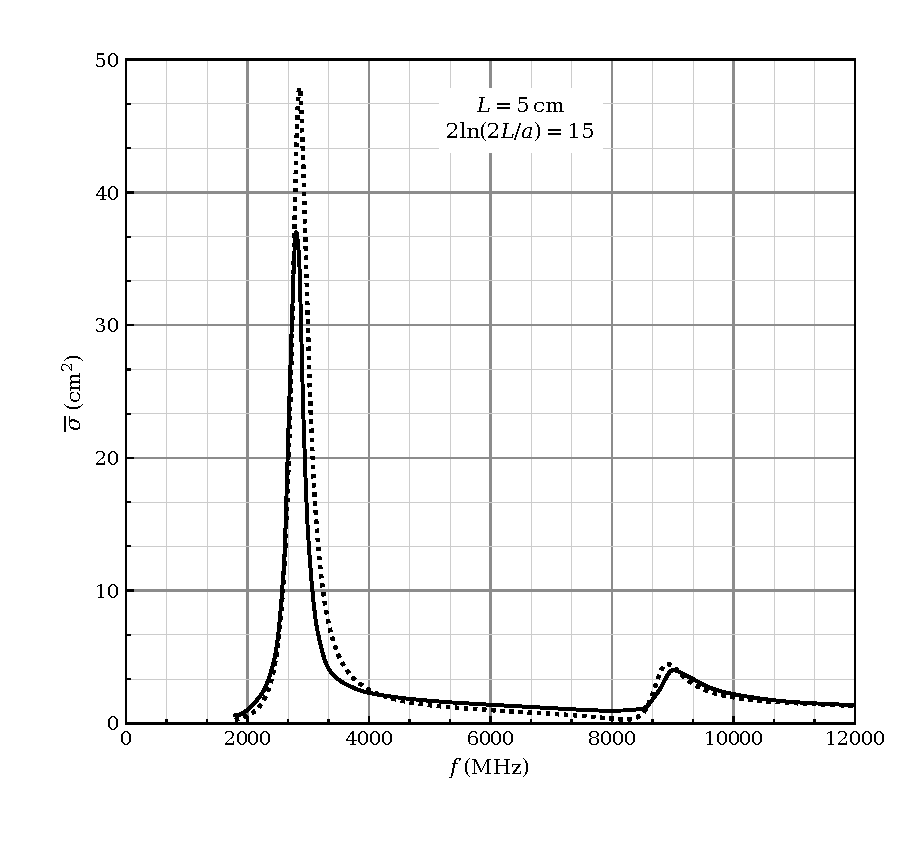
\includegraphics[width=.98\linewidth]{images/recreated/r-0228-fig78.pdf}\par\medskip
\raggedright Figure 78. The effective scattering area of a vibrator as a function of the frequency $f=c/\lambda\cdot10^{-6}$ (in megahertz) with normal incidence of a plane wave. The designations are the same as those in Figure 77.
\par\bigskip
In Figure 79 and 80 radar diagrams are constructed for vibrators of a length $L=0.5\lambda$ and $L=2\lambda$ with the specified value $L/a=900$. Curves 1 were calculated by Tai using the variational method [87]. Curves 3 were obtained by the method of induced emf [86]; curves 4 were obtained by the above-indicated method of Van Vleck. The results of calculations based on our Equations (34.12), (32.08) and (32.09) are shown by curves 2.
\end{minipage}
\end{scanpage}
